\question (Fall 2013) Draw the environment diagram for the folowing code.

\begin{minipage}{\textwidth}
\begin{lstlisting}
def miley(ray):
    def cy():
        def rus(billy):
            nonlocal cy
            cy = lambda: billy + ray
            return [1, billy]
        if len(rus(2)) == 1:
            return [3, 4]
        else:
            return [cy(), 5]
    return cy()[1]

billy = 6
miley(7)

\end{lstlisting}
\end{minipage}

\begin{solution}[0.5in]
\begin{center}
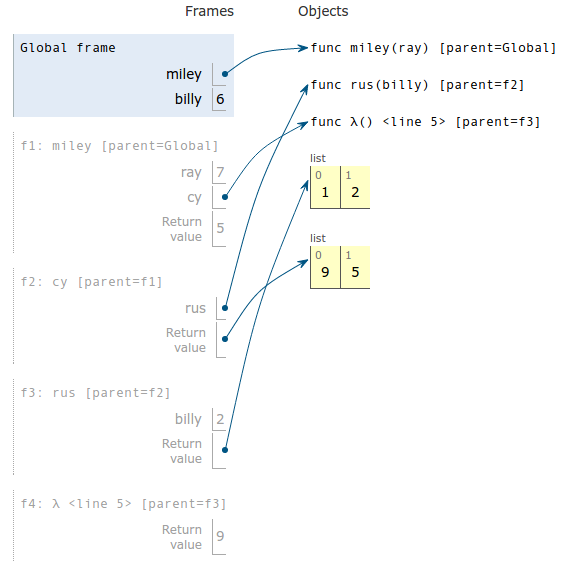
\includegraphics[scale=.5]{cyrus.png}
\end{center}
\end{solution}
